\documentclass{standalone}

\usepackage[latin1]{inputenc}
\usepackage{amsmath}
\usepackage{amssymb}
\usepackage{amsthm}

\usepackage{tikz}
\usetikzlibrary{arrows}

%% generates a tightly fitting border around the work
%\usepackage[active,tightpage]{preview}
%\PreviewEnvironment{tikzpicture}
%\setlength\PreviewBorder{0.5mm}
%%\renewcommand\PreviewBbAdjust{-\PreviewBorder 1mm -1.15mm -0.85mm}

\usepackage{color}

%\pagestyle{empty}

\begin{document}

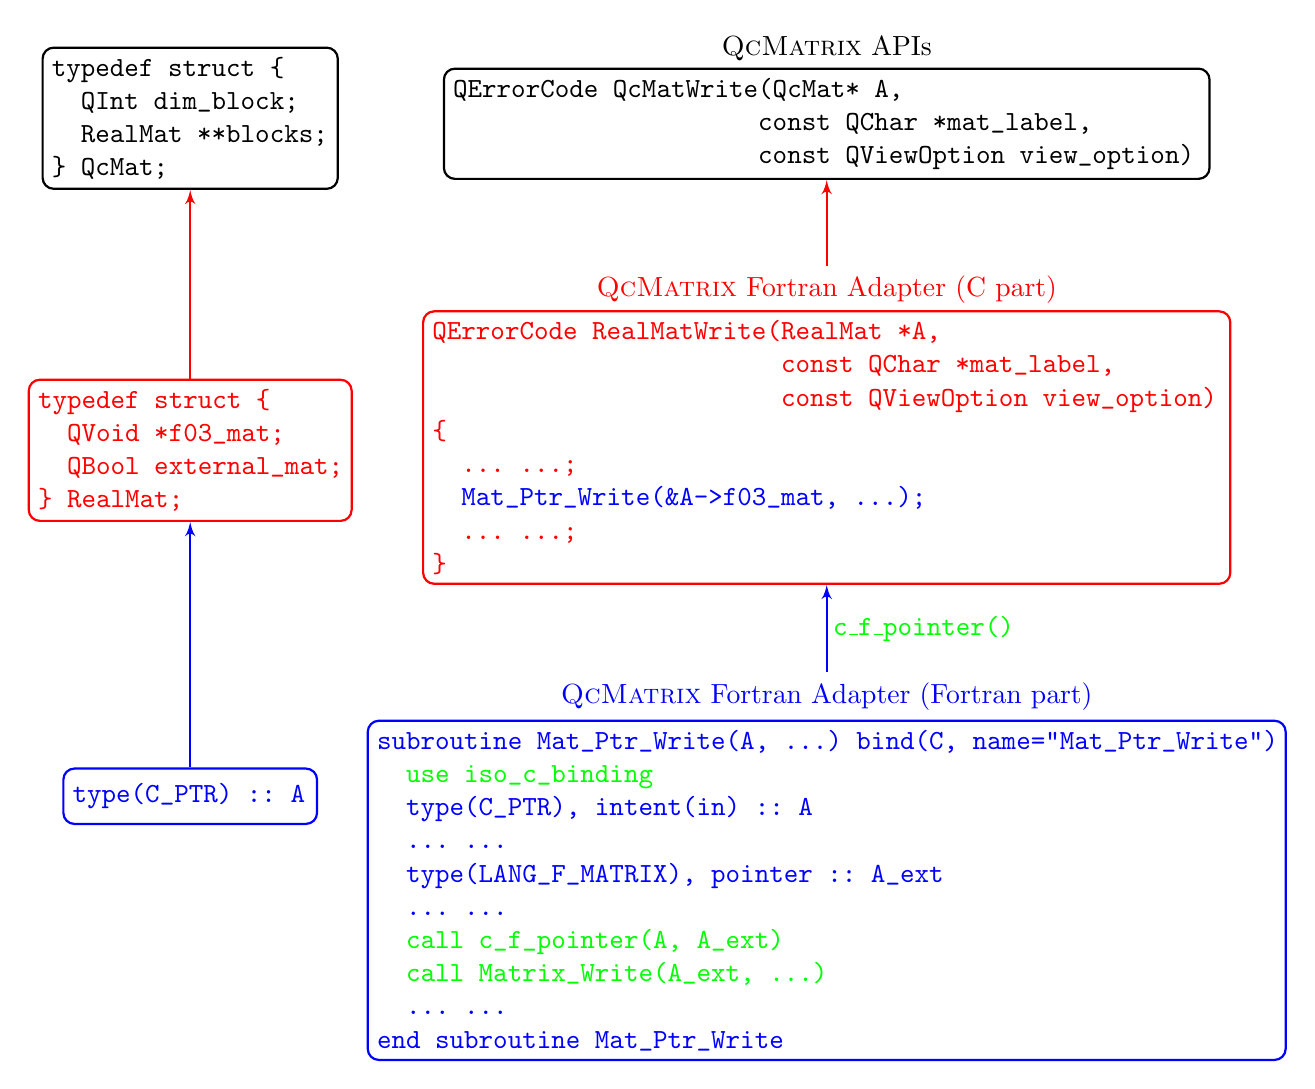
\begin{tikzpicture}[thick]
  % QcMat
  \node[color=black, rectangle, draw, text badly ragged, rounded corners, %
        minimum height=20, text width=100] (QcMatDef) %
       {\verb|typedef struct {| %
        \linebreak\verb|  QInt dim_block;| %
        \linebreak\verb|  RealMat **blocks;| %
        \linebreak\verb|} QcMat;|};
  % RealMat
  \node[color=red, rectangle, draw, text badly ragged, rounded corners, minimum height=20,
        text width=110, below of=QcMatDef, node distance=120] (RealMatDef) %
       {\verb|typedef struct {| %
        \linebreak\verb|  QVoid *f03_mat;| %
        \linebreak\verb|  QBool external_mat;| %
        \linebreak\verb|} RealMat;|};
  \draw [color=red, -latex'] (RealMatDef)--(QcMatDef);
  % type(C_PTR)
  \node[color=blue, rectangle, draw, text badly ragged, rounded corners, minimum height=20,
        text width=85, below of=RealMatDef, node distance=125] (MatPtrDef) %
       {\verb|type(C_PTR) :: A|};
  \draw [color=blue, -latex'] (MatPtrDef)--(RealMatDef);
  % APIs
  \node[color=black, right of=QcMatDef, node distance=230, yshift=25] (NoteAPIs) %
       {\textsc{QcMatrix} APIs};
  \node[color=black, rectangle, draw, text badly ragged, rounded corners, minimum height=20, % 
        text width=270, below of=NoteAPIs, node distance=27] (APIs) %
       {\verb|QErrorCode QcMatWrite(QcMat* A,| %
        \linebreak\verb|                     const QChar *mat_label,| %
        \linebreak\verb|                     const QViewOption view_option)|};
  % adapter
  \node[color=red, below of=APIs, node distance=60] (NoteAdapterC) %
       {\textsc{QcMatrix} Fortran Adapter (C part)};
  \node[color=red, rectangle, draw, text badly ragged, rounded corners, minimum height=20, % 
        text width=285, below of=NoteAdapterC, node distance=57] (AdapterC) %
       {\verb|QErrorCode RealMatWrite(RealMat *A,| %
        \linebreak\verb|                        const QChar *mat_label,| %
        \linebreak\verb|                        const QViewOption view_option)| %
        \linebreak\verb|{| %
        \linebreak\verb|  ... ...;| %
        \linebreak\color{blue}\verb|  Mat_Ptr_Write(&A->f03_mat, ...);| %
        \linebreak\color{red}\verb|  ... ...;|
        \linebreak\verb|}|};
  \node[color=blue, below of=AdapterC, node distance=90] (NoteAdapterF) %
       {\textsc{QcMatrix} Fortran Adapter (Fortran part)};
  \node[color=blue, rectangle, draw, text badly ragged, rounded corners, minimum height=20, % 
        text width=325, below of=NoteAdapterF, node distance=70] (AdapterF) %
       {\verb|subroutine Mat_Ptr_Write(A, ...) bind(C, name="Mat_Ptr_Write")| %
        \linebreak\color{green}\verb|  use iso_c_binding| %
        \linebreak\color{blue}\verb|  type(C_PTR), intent(in) :: A| %
        \linebreak\verb|  ... ...| %
        \linebreak\verb|  type(LANG_F_MATRIX), pointer :: A_ext| %
        \linebreak\verb|  ... ...| %
        \linebreak\color{green}\verb|  call c_f_pointer(A, A_ext)| %
        \linebreak\verb|  call Matrix_Write(A_ext, ...)| %
        \linebreak\color{blue}\verb|  ... ...| %
        \linebreak\verb|end subroutine Mat_Ptr_Write|};
  \draw [color=red, -latex'] (NoteAdapterC)--(APIs);
  \draw [color=blue, -latex'] (NoteAdapterF) %
        edge node[midway, xshift=35]{\color{green}\texttt{c\_f\_pointer()}}(AdapterC);
\end{tikzpicture}

\end{document}
